\chapter{Definizione del Datawarehouse}

L'obiettivo del data warehouse in oggetto è quello di fornire dati relativi
all'utilizzo di veicoli elettrici noleggiati dalla compagnia Helbiz, nel corso
della giornata, al variare delle condizioni meteo e in presenza o assenza di uno
sciopero.
L'architettura scelta è quella a tre livelli, che vede un primo livello costituito
dalle tre sorgenti operative Helbiz, Torinometeo e Scioperi, un secondo livello
costituito consistente nell'ODS ed un terzo livello costituito dai data mart.

\section{Carico di lavoro}
\begin{table}[h]
\centering
\begin{tabular}{|l|l|}
\hline
\rowcolor[HTML]{3166FF} 
{\color[HTML]{FFFFFF} \textbf{Fatto}} & {\color[HTML]{FFFFFF} \textbf{Interrogazione}}                                  \\ \hline
                                      & Numero di utilizzi durante uno sciopero nelle ore di punta                      \\ \cline{2-2} 
                                      & Numero di utilizzi durante una giornata di pioggia                              \\ \cline{2-2} 
                                      & Numero di utilizzi durante le fasce orarie lavorative                           \\ \cline{2-2} 
                                      & Numero di utilizzi durante le fasce orarie lavorative                           \\ \cline{2-2} 
                                      & Delta del numero di utilizzi tra una giornata di sciopero e una non di sciopero \\ \cline{2-2} 
                                      & Delta del numero di utilizzi tra una giornata di pioggia e una di sole          \\ \cline{2-2} 
\multirow{-7}{*}{Utilizzo veicolo}    & Delta del numero di utilizzi tra una gioranta di pioggia e una di sciopero      \\ \hline
\end{tabular}
\end{table}

\section{Progettazione concettuale}

Prodotto della fase di progettazione concettuale è il Data Fact Model di figura
\ref{fig:dfm} che modella il fatto relativio all'\textbf{utilizzo di un veicolo}.

\begin{figure}[H]                                                                                                                                                            
\centering                                                                                                                                                                   
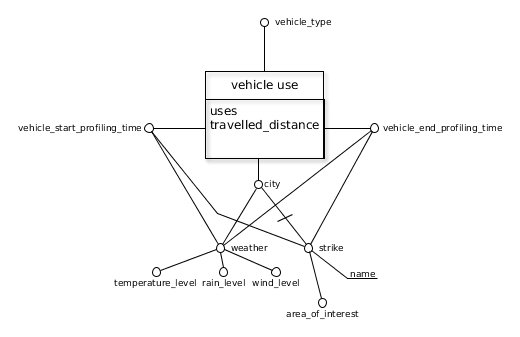
\includegraphics[width=\textwidth]{diagrams/dfm}                                                                                                                                   
\caption{DFM Vehicle use}                                                                                                                                            
\label{fig:dfm}                                                                                                                                                           
\end{figure}

Osservando il DFM si nota che gli attributi \textit{uses} e \textit{travelled\_distance} risultano
essere le misure scelte per il fatto in questione. Esse sono attributi di tipo numerico e
rappresentano rispettivamente il numero di utilizzi e la distanza percorsa mediante un determinato
veicolo.
Un'istanza di fatto è identificata dalla seguenti dimensioni:
\begin{itemize}
\item \textit{start\_profiling} e \textit{end\_profiling:} dimensioni di tipo data relative
rispettivamente all'istante di inizio e di fine di una finestra di profilazione; come è possibile
notare essi condividono la gerarchia che parte dall'attributo date e comprende tutti gli 
attributi discendenti quali \textit{day}, \textit{month}, \textit{year}, \textit{minute} e
\textit{hour};
\item \textit{vehicle\_type:} dimensione di tipo stirnga che permette la selezione tra diversi
tipi di veicoli all'interno di una finestra di profilazione;
\item \textit{city:} dimensione di tipo stringa caratterizzata dall'attributo descritto di tipo
stringa \textit{name}.
\end{itemize}

\section{Progettazione Logica e Fisica}
In questa Sezione viene descritto il processo di trasformazione del DFM, descritto al paragrafo precedente, in modello logico. 
Innanzitutto va specificato che è stata applicata la tecnica ROLAP (Relational On-Line Analytical Processing) che prevede l’utilizzo di un
modello relazionale per la rappresentazione dei dati multidimensionali.
